\section{Model adaptation}
\label{sec:model_adaptation}

\subsection{Changes to the model}
\label{subsec:changes_to_the_model}

For the purposes of this dissertation --- to perform \gls{vcr} tasks using the \gls{snmn} architecture --- several adaptations and modifications were needed to the model.
As a base, the \gls{vqa} implementation of the model is used since it most closely matches the \gls{vcr} dataset in terms of data architecture (the Clevr implementation, like the dataset, is mainly focused on benchmarking the performance of \gls{vqa} on synthetic images, whereas the \gls{vqa} and \gls{vcr} datasets represent plausible real-life settings).

The biggest difference between the original implementation and the current implementation comes from the \gls{vcr} dataset using single-choice questions instead of open-ended questions with one-word answers.
This question type is incompatible with the original loss function of the program.
The original loss function used a softmax cross-entropy over the whole vocabulary.
The new loss function uses a sigmoid cross-entropy over a probability score of 0 to 1 for each combination of question and answers.
In other words, for each \gls{vcr} task with one question and four possible answers, the loss function will expect four probability scores, with the score closest to 1 being given to the correct answer.
The reason this loss function was chosen is that it is the most suitable loss function to use for our model since its output is a \gls{logit} for answer correctness (we only need a 1 or 0 to represent whether the answer is likely to be correct or not).
Therefore, to provide the needed scores for the loss function, the model is modified to accept both a question and a possible answer, and output a confidence score between 0 and 1 whether the given answer to the given question is likely to be correct.

Aside from the answer prediction loss, there is another value which needs to be scored; the module layouts.
To predict each answer, the model needs to assemble a layout of modules to arrive at the answer.
Since the answer is dependent on the layout, the correct answer would depend upon a 'correct' layout as well.
While there is the possibility of achieving the correct answer without the 'correct' layout, the possibility is much higher when using the right or 'correct' layout.
To ensure the model uses the right layout, a \gls{softmax} loss function is chosen which takes the softmax vectors across all module \glspl{logit} and combines it with the answer loss to achieve the total loss metric.
Equation \ref{eq:vcr_loss} shows how the total loss is calculated as the product of the two weighted loss functions above, added to the weighted \gls{l2loss} of all model weight parameters.
The model will therefore train itself to match its layouts with the expert layout, consequently increasing the accuracy of the answer predictions.

\begin{equation}\label{eq:vcr_loss}
    L=(L_{ans}w_{ans}) + (L_{layout}w_{layout}) + w_{decay} \cdot L_{l2\_loss}
    % \captionsource(\gls{vcr} model loss function){The loss function used by the model during training.}{Original work written for this dissertation}
\end{equation}

Since the questions are single-choice, the model would need to look at each answer as if it were part of the question.
To support this, the model encodes both the question and the answer as input.
When first attempted, both were concatenated together and fed into the same \gls{lstm} as the original model.
This was later reworked to feed the question and answer into two \glspl{lstm}, allowing each \gls{lstm} to be tuned independently according to the question and answer.
On top of this, the model had to be modified to understand the length of the answer token sequence since it is now reliant on a new input source (the answer-fed \gls{lstm}).
Doing this prevented the model from assuming the answer to be always of fixed arbitrary length, which would make it assume the answer almost always ended with multiple 'null' tokens and thus deteriorate its performance.

\begin{figure}[htbp]
    \centering
    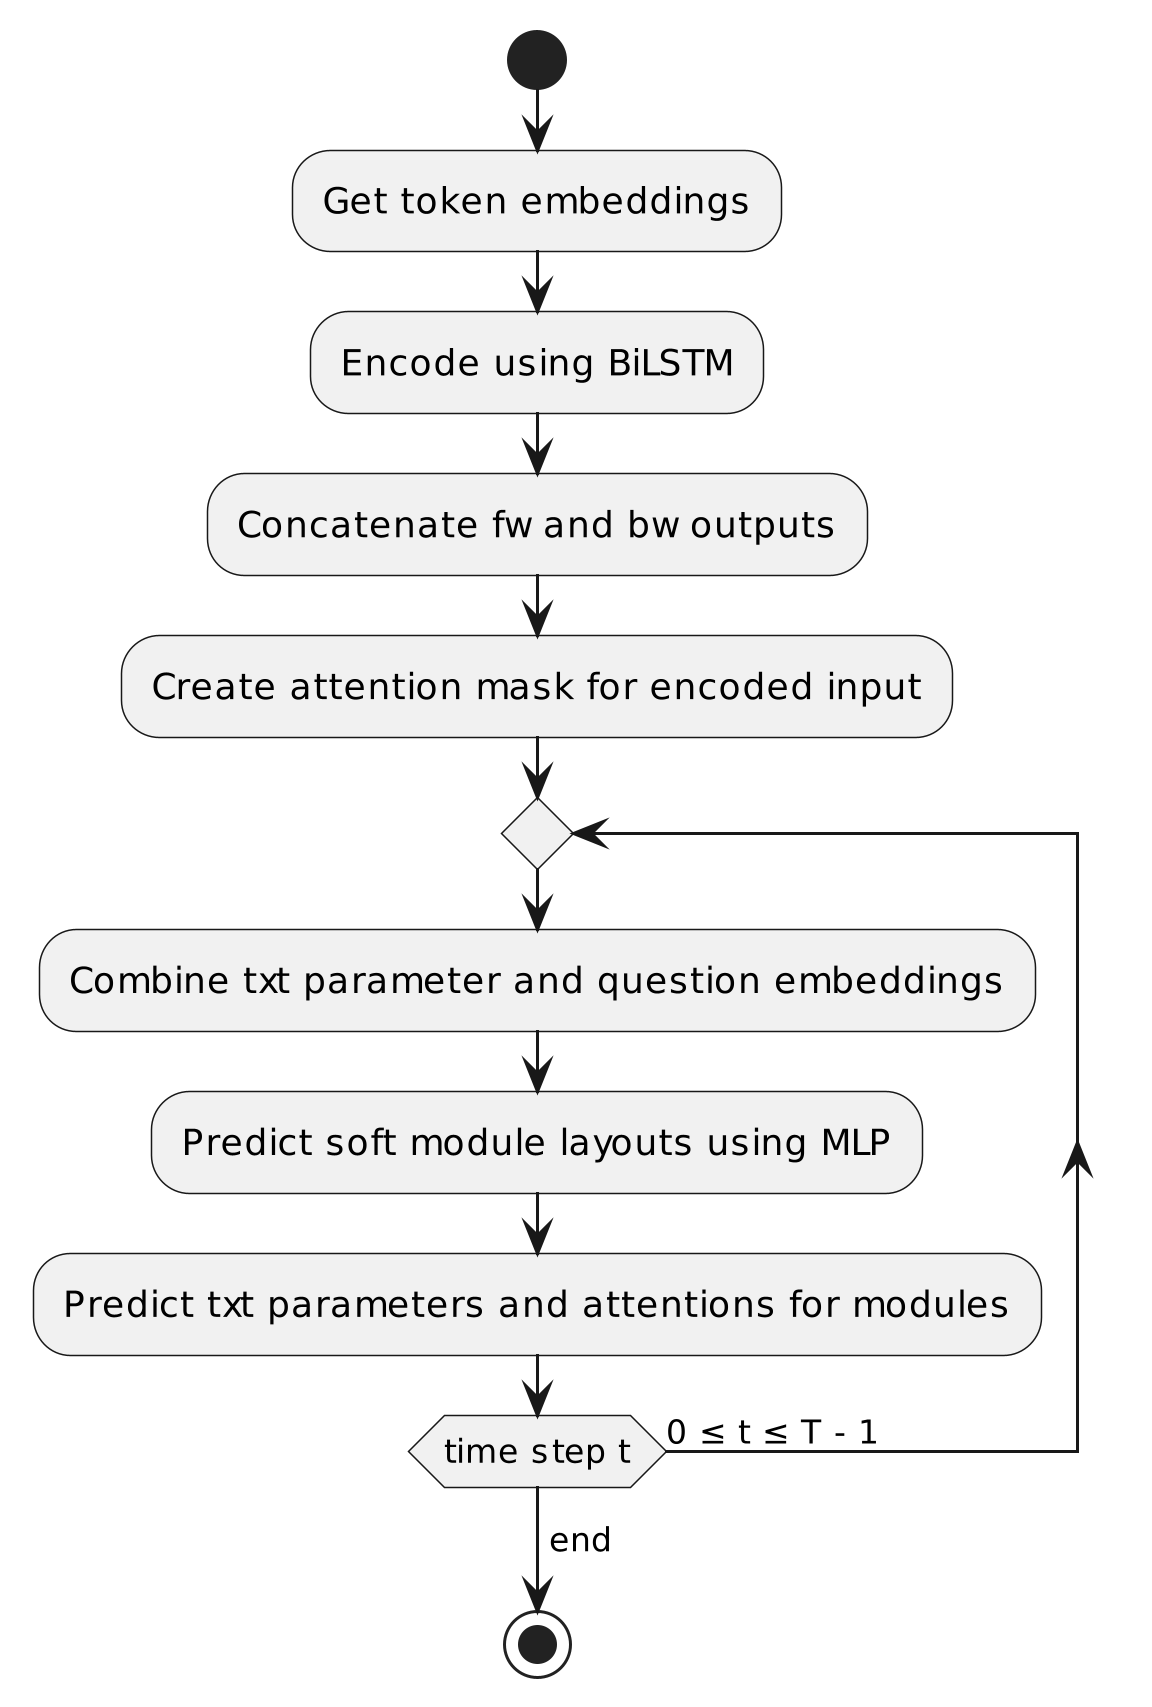
\includegraphics[width=.55\textwidth,keepaspectratio]{content/chapters/methodology/model_adaptation/figures/controller-layout-base-snmn.png}
    \captionsource(Base \gls{snmn} \gls{nas} implementation){Flow diagram of how the \gls{snmn} converts the input question to a layout.\label{fig:base_snmn_input_unit}}{Original diagram prepared for this dissertation}
\end{figure}

\begin{figure}[htbp]
    \centering
    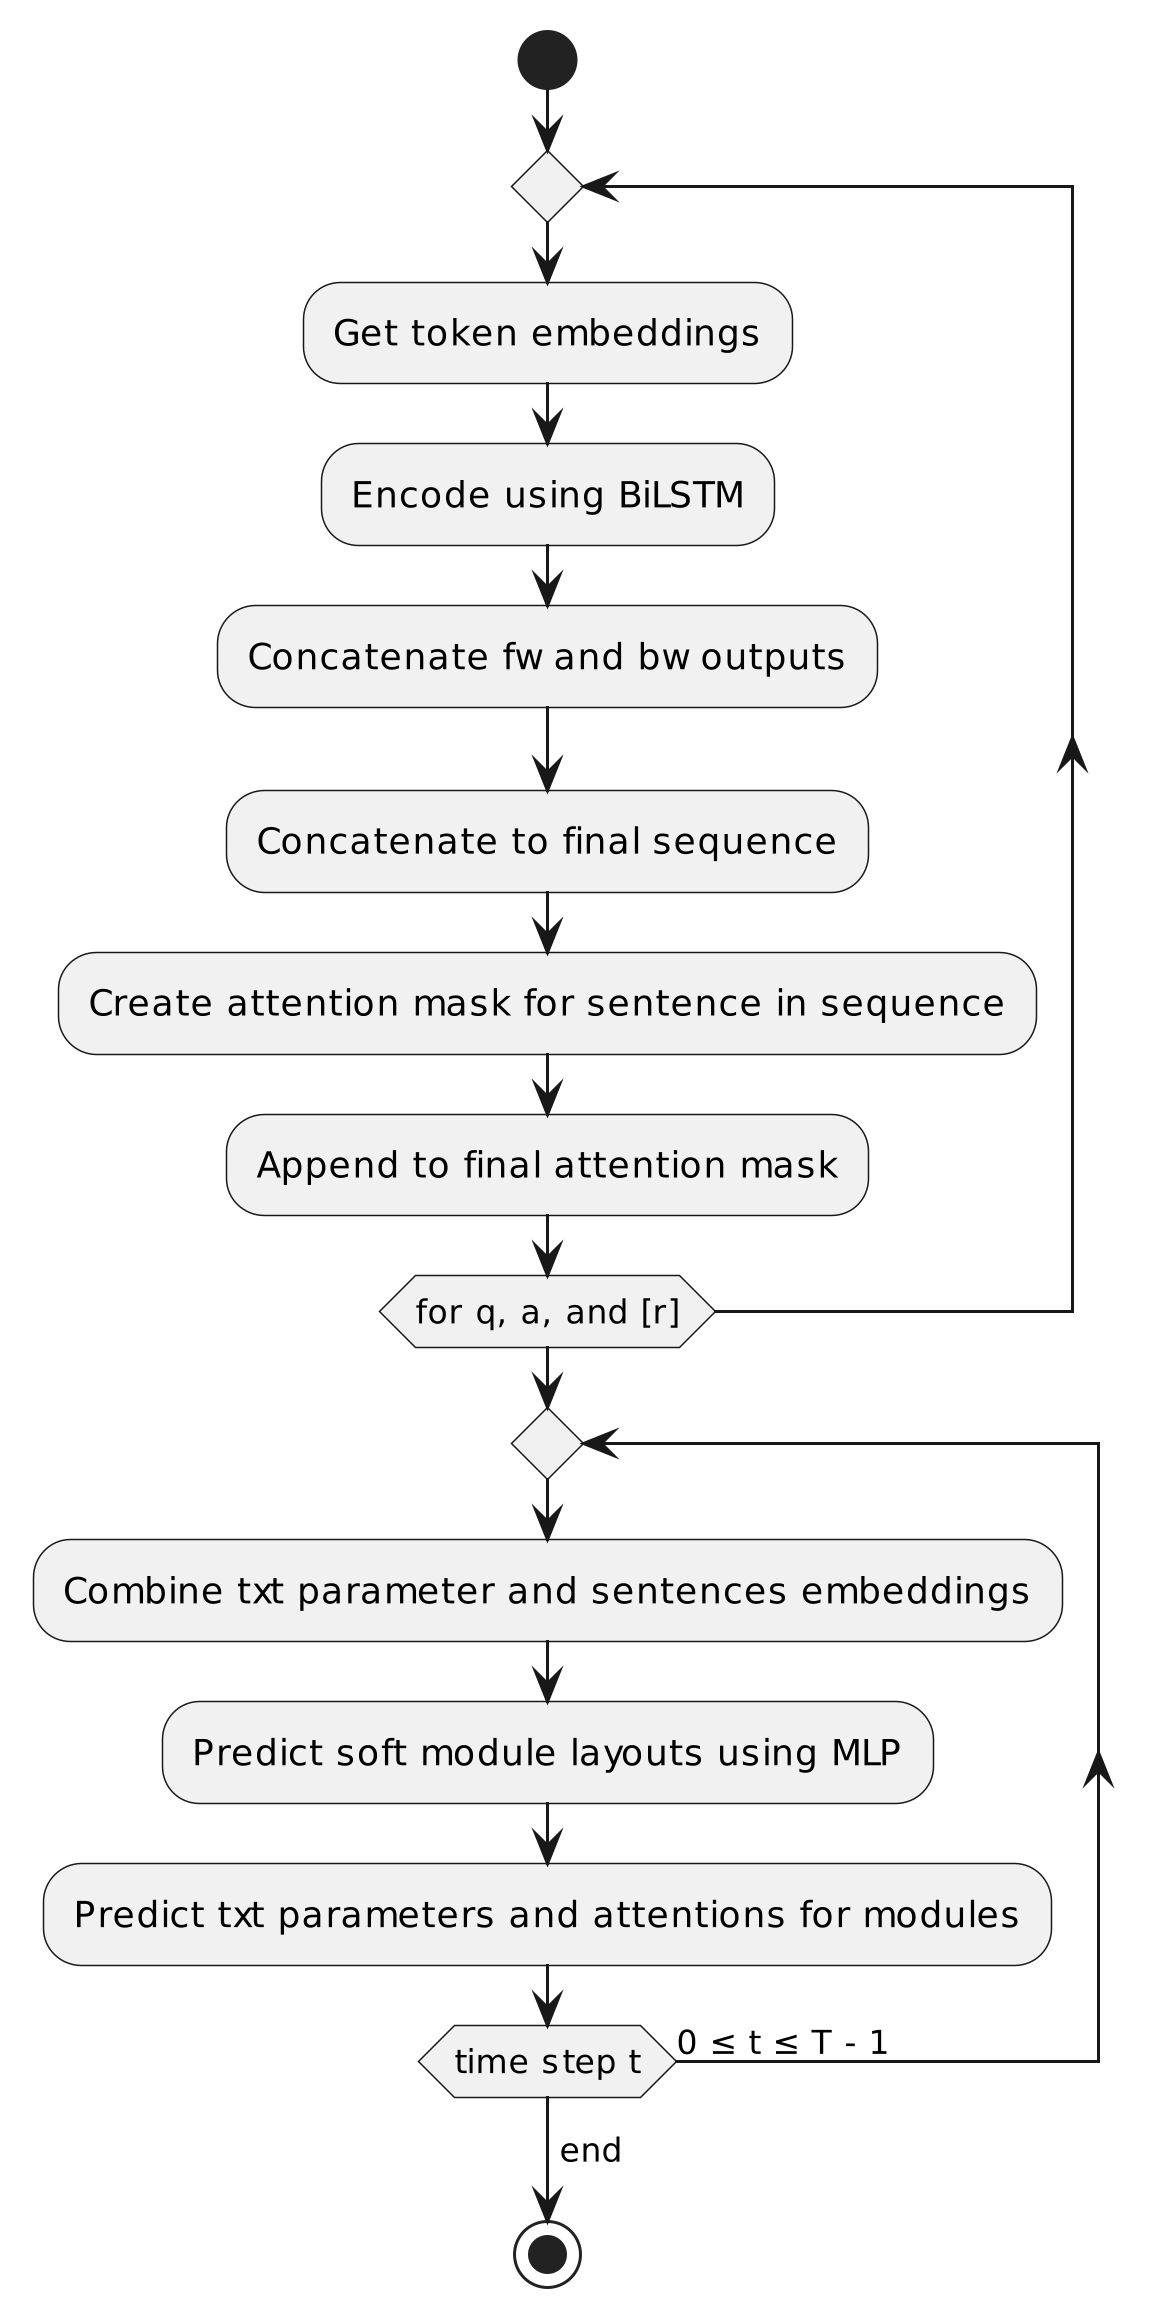
\includegraphics[width=.55\textwidth,keepaspectratio]{content/chapters/methodology/model_adaptation/figures/controller-layout-vcr-snmn.png}
    \captionsource(Modified \gls{snmn} \gls{nas} implementation){Flow diagram of how the \gls{vcr}-adapted \gls{snmn} converts the input question, answer, and rationale to a layout. Note that the rationale is only used when answering \gls{vcr} questions in QAR mode.\label{fig:vcr_snmn_input_unit}}{Original diagram prepared for this dissertation}
\end{figure}

\todo[inline]{The adaptation is out-of-date, and needs to be updated accordingly to reflect the modifications made.}

% Explain the training process (loading of data, initialisation of model, splitting of question and answer into pairs, setting of 0 or 1 if answer is correct, etc.)
